% Form 146 Copilot: brief for the Tresata take-home. Compile with: tectonic brief.tex
\documentclass[10pt,a4paper]{article}
\usepackage[a4paper,top=16mm,bottom=17mm,left=17mm,right=17mm,headheight=12pt,footskip=9mm]{geometry}
\usepackage{fontspec}
\usepackage[default]{sourcesanspro}
\usepackage{sourcecodepro}
\usepackage{xcolor,graphicx,tikz,booktabs,tabularx,enumitem,titlesec,fancyhdr,array,ragged2e,microtype}
\usepackage[most]{tcolorbox}
\usepackage{needspace}
\usepackage[hidelinks]{hyperref}
\usetikzlibrary{positioning,arrows.meta,calc,fadings,shapes.misc}

\definecolor{ink}{HTML}{1B2230}\definecolor{muted}{HTML}{5B6474}\definecolor{line}{HTML}{D9DDE4}
\definecolor{wash}{HTML}{F4F5F8}\definecolor{ai}{HTML}{5A49C8}\definecolor{rules}{HTML}{0D6E5F}\definecolor{ca}{HTML}{B42318}
\definecolor{aiwash}{HTML}{EFEDFB}\definecolor{ruleswash}{HTML}{E8F3F1}\definecolor{cawash}{HTML}{FBECEB}\definecolor{gold}{HTML}{B0892C}
\color{ink}
\hypersetup{colorlinks=true,linkcolor=ink,urlcolor=ai,citecolor=ai}

\setlength{\parindent}{0pt}\setlength{\parskip}{3.2pt}
\linespread{1.04}
\setlist{nosep,leftmargin=12pt,itemsep=1.6pt,topsep=2pt}
\setlist[itemize]{label={\color{muted}\small\textbullet}}

\titleformat{\section}{\large\bfseries\color{ink}}{\color{ca}\thesection\hspace{6pt}}{0pt}{}[\vspace{-2pt}{\color{line}\titlerule[0.8pt]}]
\titlespacing*{\section}{0pt}{9pt}{4pt}
\titleformat{\subsection}{\normalsize\bfseries\color{ink}}{}{0pt}{}
\titlespacing*{\subsection}{0pt}{5pt}{1.5pt}

\pagestyle{fancy}\fancyhf{}
\renewcommand{\headrulewidth}{0pt}
\fancyfoot[L]{\scriptsize\color{muted}Form 146 Copilot \,·\, Tresata take-home \,·\, November 2026}
\fancyfoot[R]{\scriptsize\color{muted}\thepage}
\fancypagestyle{banner}{\fancyhf{}\fancyfoot[L]{\scriptsize\color{muted}Form 146 Copilot \,·\, Tresata take-home \,·\, November 2026}\fancyfoot[R]{\scriptsize\color{muted}\thepage}}

\newcommand{\lane}[2]{\textcolor{#1}{\textbf{#2}}}
\newcommand{\kpi}[3]{\begin{tabular}[t]{@{}l@{}}{\Large\bfseries #1}\\[-1pt]{\scriptsize\color{muted}#2}\\[-2pt]{\scriptsize\color{muted}#3}\end{tabular}}
\newtcolorbox{keybox}{colback=wash,colframe=wash,arc=3pt,boxrule=0pt,left=7pt,right=7pt,top=5pt,bottom=5pt,borderline west={2.5pt}{0pt}{ca}}
\newcolumntype{L}{>{\RaggedRight\arraybackslash}X}
\newcommand{\shot}[1]{{\setlength{\fboxsep}{0pt}\setlength{\fboxrule}{0.6pt}\color{line}\fbox{\includegraphics[width=\dimexpr\linewidth-1.2pt\relax]{#1}}}}
\renewcommand{\arraystretch}{1.18}

\begin{document}
\thispagestyle{banner}

% ---------- banner ----------
\begin{tikzpicture}[remember picture,overlay]
  \node[anchor=north,inner sep=0] (b) at (current page.north) {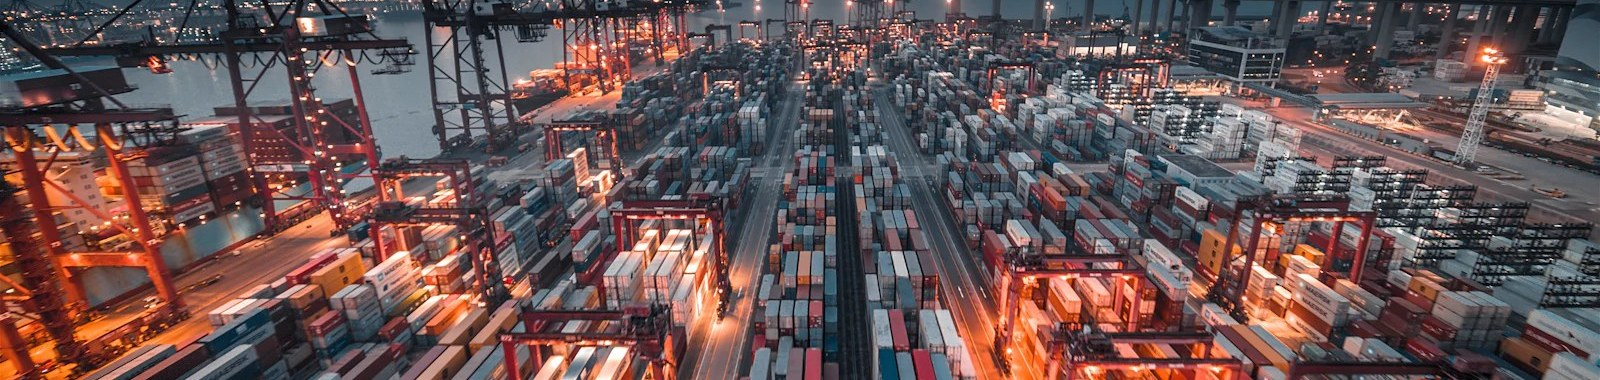
\includegraphics[width=\paperwidth,height=46mm]{img/banner.jpg}};
  \fill[ink,opacity=0.62] (b.south west) rectangle (b.north east);
  \node[anchor=south west,text width=0.86\paperwidth,align=left,inner sep=0] at ($(b.south west)+(17mm,7mm)$) {%
    {\color{white}\scriptsize\bfseries\MakeUppercase{Tresata take-home \,·\, India \,·\, Income-tax Act 2025}}\\[3pt]
    {\color{white}\fontsize{20}{23}\selectfont\bfseries Form 146 Copilot}\\[2pt]
    {\color{white!88!ink}\large Drafting treaty withholding certificates for Indian payments abroad:\\ models read, code computes, a chartered accountant decides.}};
  \node[anchor=south east,inner sep=0] at ($(b.south east)+(-4mm,1.6mm)$) {\color{white!70!ink}\tiny Photo: Unsplash};
\end{tikzpicture}
\vspace*{36mm}

{\small\color{muted}
\textbf{Prototype} \href{https://form146-copilot.vercel.app}{form146-copilot.vercel.app} \quad
\textbf{Code} \href{https://github.com/mohit-gautam7/form146-copilot}{github.com/mohit-gautam7/form146-copilot} \quad
\textbf{Scope} five treaties: US, UK, Singapore, Germany, Netherlands\par}
\vspace{2pt}

\section{The area, and what surprised me}
When an Indian company pays a non-resident for software, consulting or a licence, it must withhold Indian tax before the money leaves. If the payment is taxable and above ₹5 lakh, a chartered accountant (CA) certifies what the payment is, which treaty article applies and the rate. Since 1 April 2026 that certificate is \textbf{Form 146} (formerly 15CB), filed with the remitter's Form 145 (formerly 15CA), under the Income-tax Act 2025 \cite{faqforms}.
\begin{itemize}
  \item \textbf{The same service is taxed differently by treaty.} Consulting that leaves no lasting know-how with the payer is ``fees for technical services'' at 10\% under India--Germany \cite{de}, but business profits (no Indian tax without a permanent establishment, PE) under the US, UK and Singapore treaties, which add a ``make available'' test \cite{us,uk,sg}. The answer turns on contract wording, not the invoice label.
  \item \textbf{One payment can straddle two Acts.} TDS follows the earlier of credit and payment \cite{faqtds}; the remittance forms follow the payment date \cite{faqforms}. An amount credited on 25 March 2026 and wired on 9 April is taxed under the 1961 Act but reported on Form 146.
  \item \textbf{Treaties change quietly.} The first plan assumed the Netherlands treaty had no make-available test; the official text shows Notification S.O.\,693(E) of 1999 inserted one \cite{nl}. A most-favoured-nation clause does not apply by itself without a notification \cite{nestle}.
  \item \textbf{From the practitioner interview (Annex A):} the slow part is not arithmetic. Active time goes into reading the contract and statement of work; elapsed time goes into chasing tax residency certificates (TRC) and Form 41 \cite{form41}.
\end{itemize}

\section{The problem}
\begin{tabularx}{\linewidth}{@{}>{\bfseries}p{31mm}L@{}}
\toprule
Who & A CA who certifies foreign remittances, and the payer's finance team waiting for the certificate.\\
The task & Read the contract and invoice; decide what the payment is (royalty, technical services, business profits, reimbursement); check the treaty article and its conditions; compute the rate; sign Form 146.\\
How often & The CA I interviewed signs \textbf{25--40 certificates a month}.\\
What it costs today & \textbf{30--45 minutes} for a repeat vendor, \textbf{2--4 hours} of active work for a new contract, \textbf{2--5 days} elapsed when documents are missing. A wrong certificate leaves the payer liable for the unpaid tax with interest and puts the CA's signature at risk.\\
Why now & The new Act and forms started on 1 April 2026. Templates are moving from 15CB to 146, and payments credited before and paid after the change follow two Acts at once.\\
\bottomrule
\end{tabularx}
\vspace{2pt}
\begin{keybox}
\textbf{Problem statement.} Working out whether a cross-border payment is a royalty, technical services or business profits under the right treaty is slow judgement work, repeated from scratch for every certificate. Since April 2026 it must be done under renumbered law while old templates are still in circulation, and a confident mistake costs the payer tax and interest.
\end{keybox}
\textbf{Out of scope:} filing on the tax portal and the UDIN; profit attribution to a PE; beneficial-ownership, principal-purpose and multilateral-instrument analysis; the yearly aggregate for the ₹5 lakh threshold (applied per payment); countries beyond the five treaties; PDF upload (text only); tax advice: the CA decides.

\section{Solution design}
The design splits the work by what each part can be trusted with: \lane{ai}{models read}, \lane{rules}{code computes}, \lane{ca}{a CA decides}. The three lanes never mix: a model never produces a rate, and code never decides what a contract means.

\begin{center}
\begin{tikzpicture}[font=\scriptsize,
  box/.style={rounded corners=3pt,draw=#1,line width=0.9pt,fill=#1!7,align=left,inner sep=5pt,anchor=north west},
  inbox/.style={rounded corners=3pt,draw=ink!70,fill=wash,align=left,inner sep=5pt,anchor=north west,text width=26mm},
  ar/.style={-{Stealth[length=5pt]},line width=0.8pt,color=ink!80}]
  \node[inbox] (docs) at (0,0) {\textbf{Documents}\\contract, invoice\\{\color{muted}untrusted text}\\[3pt]\textbf{Treaty text}\\{\color{muted}official, per country}};
  \node[inbox] (facts) at (0,-2.85) {\textbf{Facts the CA vouches for}\\{\color{muted}credit \& payment dates, amount, TRC, Form 41, PAN, payee type}};
  \node[box=ai,text width=36mm] (ai) at (3.55,0.15) {{\color{ai}\textbf{AI lane} \,·\, probabilistic}\\3 model families vote\\{\color{muted}Groq \,·\, NVIDIA NIM \,·\, OpenRouter}\\fixed labels only: category, make-available, PE risk, \textbf{verbatim quotes}\\{\color{muted}fallback: next family if one is down}};
  \node[box=rules,text width=36mm] (chk) at (3.55,-2.75) {{\color{rules}\textbf{Quote check + vote} \,·\, code}\\quote must exist in the source\\agree / flag / contested / abstain\\{\color{muted}fewer than 2 verified votes $\to$ abstain}};
  \node[box=rules,text width=38mm] (eng) at (8.25,-0.35) {{\color{rules}\textbf{Rules lane} \,·\, exact}\\pure function over \texttt{rules.json}\\{\color{muted}each rule: source quote, effective dates, last verified}\\Act by date \,·\, treaty vs Act rate\\surcharge, cess, MFN, no-PAN, gross-up\\every reading computed\\{\color{muted}stale rule $\to$ refuses; every step traced}};
  \node[box=ca,text width=34mm] (ca) at (13.15,-0.35) {{\color{ca}\textbf{CA lane} \,·\, accountable}\\sees votes, quotes, trace\\signs, overrides with a reason, or sends back\\[2pt]\textbf{Draft Form 146}\\{\color{muted}each field shows who supplied it}\\[2pt]\textbf{Hash-chained log}\\{\color{muted}SHA-256, verifiable offline}};
  \draw[ar] (docs.east|-ai.west) -- (ai.west);
  \draw[ar] (ai.south) -- (chk.north);
  \draw[ar] (chk.east) -- ++(0.35,0) |- ($(eng.west)+(0,-0.6)$);
  \draw[ar] (facts.south) -- ++(0,-0.25) -| ($(eng.south)+(0,0)$) node[pos=0.25,below,color=muted,font=\tiny]{facts go straight to the rules, never through a model};
  \draw[ar] (eng.east) -- (ca.west);
\end{tikzpicture}
\end{center}

\begin{minipage}[t]{0.485\linewidth}
\subsection{Data in, answer out}
\textbf{In:} contract and invoice text; the treaty articles for the payee's country, stored with their official source links; facts the CA vouches for. \textbf{Out:} a rate with its basis and article, the tax, the governing Act and forms, a step-by-step trace with sources, the model votes with their quotes, and a draft Form 146.
\subsection{Handling uncertainty and mistakes}
\begin{itemize}
  \item A vote counts only if it quotes both the contract and the treaty, and both quotes are found word for word in the sources.
  \item Fewer than two counted votes: \textbf{abstain}. A split between technical services and business profits is never settled by majority: it is \textbf{contested}, and the engine computes every reading for the CA.
  \item A model that is down is replaced by one from another family; an outage never counts as a vote.
  \item A stale or out-of-window rule makes the engine refuse. Unverified rules are flagged on every result that uses them.
\end{itemize}
\end{minipage}\hfill
\begin{minipage}[t]{0.485\linewidth}
\subsection{Why AI is needed, and only here}
The hard step is reading free text: a ``subscription'' that grants rights to reproduce and sublicense software is a royalty \cite{ea}; ``training our engineers to run the pipeline'' makes know-how available, while a research report does not. Keyword rules fail both ways. Everything an auditor checks (rates, dates, thresholds, arithmetic) is code, and the CA signs.
\subsection{Where the knowledge lives}
\textbf{Treaty text}: official texts with source links. \textbf{Rates and rules}: \texttt{rules.json}, each with a source quote, effective dates and a last-verified date; older than a year or outside its window, the engine refuses. \textbf{Models}: reading skill only, never the law. \textbf{The CA}: judgement and accountability.
\subsection{Traceability}
Each rate step links to its source and quote; each model claim has a verified quote; raw model replies are stored; the CA's decisions sit in a hash-chained log an auditor can re-verify offline.
\end{minipage}

\subsection{Alternatives I considered and rejected}
\begin{tabularx}{\linewidth}{@{}p{50mm}L@{}}
\toprule
\textbf{Alternative} & \textbf{Why not}\\\midrule
One LLM call returns the rate & Rates and arithmetic would not be exact or auditable, and the model cannot know a rule changed last month.\\
Retrieval with embeddings & The corpus is tiny (four articles per treaty). Looking them up by country is exact; similarity search adds a way to fetch the wrong article.\\
One model checking itself & Its errors correlate with itself. Three model families at least cancel random errors.\\
Several cooperating agents & The workflow is fixed. Agents add failure modes without adding accuracy.\\
Rules or keywords only & Cannot read contracts; fails the ``SaaS that grants copyright'' test case.\\
Majority vote wins & Rejected after evidence: in the first live run a 2--1 majority produced a wrong nil rate shown as final.\\
Escalate a split only if the readings give different tax & Tried, and rescored on the recorded answers: it fixed one over-cautious case but turned a genuinely contested case into a confident nil, because all three models misread it the same way.\\
A database server & No shared data in a demo. A local hash-chained log is verifiable; Postgres when several reviewers share a queue.\\
\bottomrule
\end{tabularx}

\needspace{24\baselineskip}
\section{Proof: 17 test cases, and where it fails}
\begin{minipage}[t]{0.50\linewidth}\vspace{0pt}
\shot{img/workbench.jpg}\\[-1pt]
{\scriptsize\color{muted}\textbf{The workbench on a contested case} (live site, recorded model answers). Two models say ``technical services, no know-how transferred'', one says ``business profits''. The rules lane computes all three readings (10\%, nil, nil) and sends the case to the CA instead of picking one.}
\end{minipage}\hfill
\begin{minipage}[t]{0.47\linewidth}\vspace{0pt}
All contracts and invoices are synthetic; the treaty texts are real. 14 cases each target one trap (SaaS, make-available, Netherlands equipment hire, MFN claim, no TRC, gross-up, old Act, PE risk, below threshold, no PAN). Three more were written to break it: a prompt injection in an invoice, a ``SaaS'' contract that grants copyright, and a credit/payment straddle across 1 April 2026. Expected answers were fixed before the models saw the cases.

The headline metric is \textbf{wrong and confident}: a wrong rate shown as final instead of being sent to the CA.

\vspace{4pt}
\kpi{17/17}{rules lane}{(regression only)}\hfill\kpi{12/17}{full pipeline}{correct}\hfill\kpi{\textcolor{rules}{0}}{wrong and}{confident}

\vspace{6pt}
\textbf{Where it fails.} All five misses went to the CA rather than giving a wrong rate. Four trace back to free-tier outages (OpenRouter's 50 requests a day) that left one verified vote. One, a UK research report, is the dispute rule being over-cautious. In the injection case neither model obeyed the injected instruction or used the fake quote; it abstained because one model misquoted the treaty. Seventeen cases cannot show the rules generalise.
\end{minipage}

\vspace{6pt}
{\small
\begin{tabularx}{\linewidth}{@{}Lccl@{}}
\toprule
\textbf{Run} (live free-tier models, 2 Nov 2026) & \textbf{Fully correct} & \textbf{Wrong \& confident} & \textbf{Notes}\\\midrule
1: first 14 cases & 11/14 & \textcolor{ca}{\textbf{1}} & 2--1 vote gave a wrong nil rate; dispute rule added\\
2: same 14, after the rule & 10/14 & 0 & 3 misses were quota outages\\
3: the 3 new cases, first contact & 1/3 & 0 & found a dispute escalated that could not change the rate\\
All 17 after that fix (what the site replays) & \textbf{12/17} & \textbf{0} & two fixes so far made on cases already seen\\
\bottomrule
\end{tabularx}}

\vspace{5pt}
\begin{minipage}[t]{0.495\linewidth}\vspace{0pt}
\shot{img/hero.jpg}\\[-1pt]
{\scriptsize\color{muted}\textbf{Landing page.} The 3D scene plays the product's own sequence: models read, rules compute, the CA seals.}
\end{minipage}\hfill
\begin{minipage}[t]{0.475\linewidth}\vspace{0pt}
\shot{img/eval.jpg}\\[-1pt]
{\scriptsize\color{muted}\textbf{Evaluation page.} The rules lane and the full pipeline are scored separately, so each failure is blamed on the right part.}
\end{minipage}

\needspace{14\baselineskip}
\section{Risks and how the design handles them}
{\small
\begin{tabularx}{\linewidth}{@{}>{\bfseries}p{31mm}L@{}}
\toprule
Wrong answers & Three-family vote, verbatim quote check, abstain and contested paths, every reading computed. Measured by ``wrong and confident'', not accuracy. The CA signs.\\
Outdated rules & Effective and last-verified dates on every rule; stale rules make the engine refuse. Two rules are still unverified (no surcharge on treaty rates; the no-PAN carve-out under the 2025 Act) and are flagged on every result. Surcharge slabs and the 2025 rate are checked against the Finance Bill 2026 \cite{fb}; the enacted Act should be compared.\\
Confidential data & Real contracts would go to third-party APIs. The prototype uses only synthetic data and the public site does not call models. For a firm: redact names and amounts, use zero-retention terms, or self-host an open model.\\
Liability & The law requires a CA's certificate, so the CA is accountable. The tool drafts and never shows ``approved''; every Form 146 field shows whether the model, the code or the CA supplied it; overrides need a reason.\\
Prompt injection & Documents are fenced as evidence; a model cannot set a rate; quotes must exist; with no TRC even an obeyed ``business profits'' goes to the CA. Tested once; one naive attack proves little.\\
\textcolor{ca}{Weakest point} & Correlated error: three models can share one misconception, and a wrong rule in \texttt{rules.json} is applied consistently. Voting catches neither. Seen already: on the contested Singapore case all three models read nil, and only the blunt dispute rule sent it to the CA. What would break it: a treaty amendment not yet in the rules file, or a contract style no test case covers.\\
\bottomrule
\end{tabularx}}

\section{Before spending more time on this}
\begin{itemize}
  \item Interview three to five more CAs and a bank's remittance desk; time real, anonymised certificates with and without the tool.
  \item Have practitioners write the test cases and expected answers, so the author of the rules is not also the examiner.
  \item Model the yearly aggregate (a payment ledger) and the AO-certificate route, where Form 146 is not needed \cite{faqforms}.
  \item Add a challenge pass for every nil result: ask a model what clause could make the payment taxable.
  \item Decide how contracts stay confidential (redaction or self-hosting) before any real contract touches it.
  \item \textbf{Another jurisdiction:} for a US payer the inputs become Form W-8BEN-E, withholding under chapter 3 and Form 1042-S, and the AI question becomes ``US-source income or not?''. The rules file changes; the three lanes do not.
\end{itemize}

{\footnotesize
\renewcommand{\refname}{\normalsize\bfseries References}
\begin{thebibliography}{99}\setlength{\itemsep}{0.5pt}
\bibitem{faqforms} Income Tax Department, \emph{Income-tax Forms FAQs} (Forms 145/146, remittance date, AO-certificate route, Q20--27). \url{https://www.incometax.gov.in/iec/foportal/help/all-topics/e-filing-services/income-tax-forms}
\bibitem{faqtds} Income Tax Department, \emph{TDS Compliance FAQs} (earlier of credit or payment, Q1). \url{https://www.incometax.gov.in/iec/foportal/help/all-topics/e-filing-services/\%20tds\%20compliance-faq}
\bibitem{form41} Income Tax Department, \emph{Form 41 User Manual} (treaty relief information, section 159). \url{https://www.incometax.gov.in/iec/foportal/newformpage/forms/form41-UM}
\bibitem{fb} \emph{The Finance Bill, 2026} (Bill No.\ 3 of 2026, as introduced in Lok Sabha), First Schedule, Part II. \url{https://www.incometax.gov.in/iec/foportal/sites/default/files/2026-03/Finance_Bill.pdf}
\bibitem{us} India--USA DTAA, Article 12 (IRS official text). \url{https://www.irs.gov/pub/irs-trty/india.pdf}
\bibitem{uk} India--UK DTAA as amended in 2013, Article 13 (GOV.UK). \url{https://assets.publishing.service.gov.uk/government/uploads/system/uploads/attachment_data/file/736294/1993_India_-_UK_Double_Taxation_Agreement__as_amended_in_2013_-_in_force.pdf}
\bibitem{sg} India--Singapore DTAA, Article 12 (CBDT). \url{https://wm.incometaxindia.gov.in/w/singapore-comprehensive-agreements-1}
\bibitem{de} India--Germany DTAA, Article 12 (CBDT). \url{https://wm.incometaxindia.gov.in/w/germany-comprehensive-agreements-1}
\bibitem{nl} India--Netherlands DTAA, Article 12 as amended by Notification S.O.\,693(E), 30 August 1999 (CBDT). \url{https://wm.incometaxindia.gov.in/w/netherlands-comprehensive-agreements-1}
\bibitem{ea} \emph{Engineering Analysis Centre of Excellence Pvt.\ Ltd.\ v.\ CIT}, Supreme Court of India, 2 March 2021 (software licences and royalty).
\bibitem{nestle} \emph{Assessing Officer v.\ Nestl\'e SA}, Supreme Court of India, 19 October 2023 (MFN clauses need a notification).
\end{thebibliography}
\vspace{2pt}{\color{muted}Photographs: Unsplash (Scott Graham, Previn Samuel, Timelab, Markus Spiske). Screenshots: the live prototype, recorded model answers, 2 November 2026. Practitioner interview: Annex A. Build chat: Annex B.}\par}

% ---------- appendix ----------
\newpage
\begin{tikzpicture}[remember picture,overlay]
  \node[anchor=north,inner sep=0] (b) at (current page.north) {
\includegraphics[width=\paperwidth,height=24mm,trim=0 330 0 330,clip]{img/signing.jpg}};
  \fill[ink,opacity=0.55] (b.south west) rectangle (b.north east);
  \node[anchor=south west,inner sep=0] at ($(b.south west)+(17mm,5mm)$) {\color{white}\fontsize{16}{19}\selectfont\bfseries Appendix: what I added beyond the AI};
  \node[anchor=south east,inner sep=0] at ($(b.south east)+(-4mm,1.6mm)$) {\color{white!70!ink}\tiny Photo: Unsplash};
\end{tikzpicture}
\vspace*{15mm}

{\small\color{muted}I used Claude (Claude Code) for research, architecture options, most of the code, the evaluation harness and drafting this brief. Groq, NVIDIA NIM and OpenRouter models are the ones under test inside the prototype. The interview record (Annex A) and the full build chat (Annex B) follow this page.\par}

\subsection{Where AI helped}
Finding and reading primary sources (the 2025 Act mapping, the treaty texts, the Income Tax Department FAQs, the Finance Bill schedule); proposing the three-lane split, the quote check and the evaluation metric; writing the Next.js prototype and tests; drafting and editing this document. Three of my prompts, verbatim:
\begin{tcolorbox}[colback=aiwash,colframe=aiwash,arc=3pt,boxrule=0pt,left=7pt,right=7pt,top=4pt,bottom=4pt,borderline west={2.5pt}{0pt}{ai},fontupper=\itshape\small]
``research for this and give me some good ideas for this \dots{} think, research, and give me a best solution''\\[2pt]
``add more option also like nvidia nim,groq,openrouter all 3 and chached replay also so give me best running''\\[2pt]
``make sure to add option of fallback if any model is not available then you can use other''
\end{tcolorbox}

\subsection{What I rejected or corrected, and how I knew}
\begin{itemize}
  \item \textbf{The Netherlands assumption.} The plan treated the India--Netherlands treaty as having no make-available test. The official text shows Notification S.O.\,693(E) of 30 August 1999 inserted it \cite{nl}, so that test case became equipment hire, which the Dutch royalty definition excludes.
  \item \textbf{Majority voting.} The first live evaluation showed a 2--1 majority producing a wrong nil rate presented as final. Majority-wins was dropped for splits that change the tax.
  \item \textbf{``One unfound quote voids the vote''.} Too strict: a non-breaking hyphen or an ellipsis threw away correct answers. Replaced by ``at least one verified quote from the document and one from the treaty'', with unfound quotes shown in red.
  \item \textbf{A wrong test, not wrong code.} A test expected 21.216\% on ₹20 lakh; surcharge only starts above ₹1 crore \cite{fb}, so the engine's 20.8\% was right.
  \item \textbf{An outage that looked like a vote.} I noticed the workbench showing a raw HTTP 429 error as if it were a model's answer. It now says ``No model answered'' with the reason.
  \item \textbf{Claims in my own research notes} (credit vs payment date, Form 41, the surcharge slabs) went into the code only after they were checked against the Income Tax Department FAQs and the Finance Bill 2026 \cite{faqtds,faqforms,form41,fb}.
\end{itemize}

\subsection{What came from me}
\begin{itemize}
  \item \textbf{The practitioner interview (Annex A).} The CA said the statement of work, not the invoice label, decides the classification; that time goes into reading contracts and chasing documents; that they would not sign without clause-level evidence and a calculation they can reproduce; and that treaty rates are applied without surcharge and cess. These shaped the quote requirement, the source trace on every step, the rule that nothing is ever marked ``approved'', and the treaty-rate rule.
  \item \textbf{Three model providers, a fallback chain and recorded replay,} so free-tier limits never break the public demo. Run 2 showed why: OpenRouter's daily cap ran out mid-run.
  \item \textbf{Three test cases written to break it:} an injection in an invoice, a ``SaaS'' contract that grants copyright, and a credit in March with payment in April 2026. The last one exposed a gap nobody had flagged: the tool escalated a dispute that could not change the rate under the Germany treaty.
\end{itemize}

\subsection{One thing I would defend live without tools}
\begin{keybox}
\textbf{Models read, code computes, a CA decides.} The rate is a lookup and arithmetic over published law, so it must be exact and traceable, and that belongs in code with a source for every number. What the payment \emph{is} depends on reading contract language, which is where models help and where they can be wrong. So their output is limited to fixed labels backed by quotes that must exist in the documents, and any disagreement that would change the tax goes to the CA with every answer computed. Three models agreeing is not proof: they can share one misconception, which is why the CA signs and why the measure that matters is how often the tool is wrong and confident, not how often it is right.
\end{keybox}

% ---------- Annex A ----------
\newpage
\begin{tikzpicture}[remember picture,overlay]
  \node[anchor=north,inner sep=0] (b) at (current page.north) {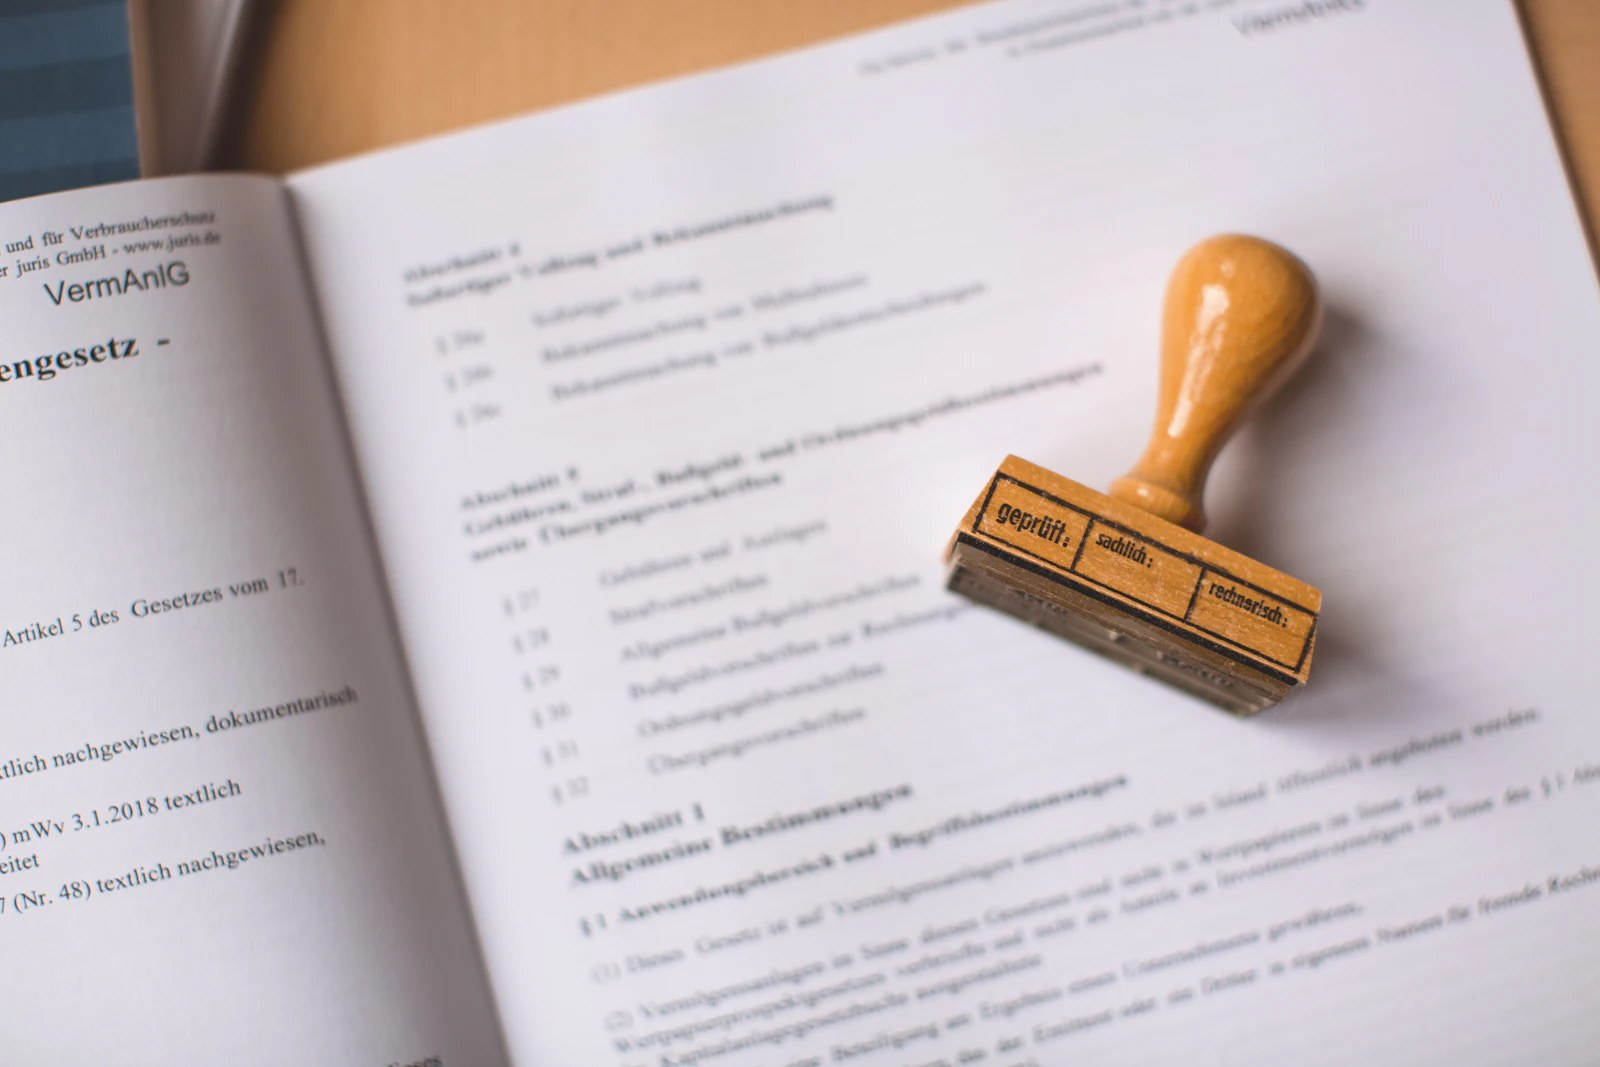
\includegraphics[width=\paperwidth,height=24mm,trim=0 380 0 330,clip]{img/stamp.jpg}};
  \fill[ink,opacity=0.55] (b.south west) rectangle (b.north east);
  \node[anchor=south west,inner sep=0] at ($(b.south west)+(17mm,5mm)$) {\color{white}\fontsize{16}{19}\selectfont\bfseries Annex A: practitioner interview};
  \node[anchor=south east,inner sep=0] at ($(b.south east)+(-4mm,1.6mm)$) {\color{white!70!ink}\tiny Photo: Unsplash};
\end{tikzpicture}
\vspace*{15mm}

{\small\color{muted}Interview with a practising chartered accountant who certifies foreign remittances for corporate clients. Answers summarised from my notes. Outside the four-page brief.\par}
\vspace{4pt}
\begin{tabularx}{\linewidth}{@{}>{\bfseries\RaggedRight}p{44mm}L@{}}
\toprule
How many certificates per month? & Roughly \textbf{25--40 Form 15CB/146 certificates a month} across regular corporate clients.\\\midrule
How long does one take? & Repeat vendor with an existing MSA: \textbf{30--45 minutes}. First-time vendor with a bespoke contract: \textbf{2--4 hours of active work}. Calendar turnaround is often \textbf{2--5 days} when documents are missing.\\\midrule
Which part takes longest? & Active time goes into reading the contract and SOW to work out what rights and services are really being paid for. Elapsed time goes into chasing a valid TRC, Form 41 (formerly Form 10F), beneficial-owner and no-PE declarations. Portal, DSC and UDIN issues add friction.\\\midrule
The last one you nearly got wrong? & A UK cloud-platform invoice labelled ``Annual Platform Subscription''. The SOW also covered custom API architecture and training on proprietary code. It was the SOW, not the invoice label, that made the reviewer ask whether technical knowledge was being made available.\\\midrule
What changed on 1 April 2026? & Forms 15CA/15CB became Forms \textbf{145/146}, Form 10F became Form \textbf{41}, and Rule 220 now governs the remittance forms. Form 146 is the equivalent of 15CB, not a verbatim copy, so old wording should not be pasted across.\\\midrule
Credit or payment: which date triggers TDS? & Whichever is earlier. If the amount is credited by 31 March 2026 and paid in April, the old Act governs the TDS; the remittance forms follow the remittance date. (This matches the Income Tax Department's FAQs \cite{faqtds,faqforms}.)\\\midrule
Would you sign a certificate a tool drafted? & Not blindly. The CA would need clause-level evidence, the exact treaty article, protocol and current notification, TRC and Form 41 validity, the beneficial-ownership and PE position, and a calculation they can reproduce.\\\midrule
Do you add surcharge and cess on a treaty rate? & No: the treaty rate is applied as the ceiling where the treaty's wording and covered-taxes article support it. Surcharge and cess apply when the domestic Act rate is used. Treaty wording should be checked treaty by treaty.\\
\bottomrule
\end{tabularx}

\vspace{6pt}
\begin{keybox}
\textbf{What changed in the prototype because of the interview.} The contract, not the invoice label, is what the models must quote; the trace shows every source so the calculation is reproducible; the tool never labels anything ``approved''; and treaty rates are applied without surcharge or cess. That last rule stays flagged as ``not verified against a statute'' in \texttt{rules.json}, because a practitioner's practice is evidence, not a primary source.
\end{keybox}

\end{document}
